\section{Data generation}

In this section, we introduce the methods for producing the divergence free and non divergence free vector fields used for training and testing.
\justin{
We know that we can't possibly present every type of divergence free or non divergence free vector field for training. Our hope is that the neural net learns what divergence free means from a small family of divergence free vector fields and is able to properly generalize these ideas. Our setup consists of a set of training data generated from a family of divergence free fields of a specific form. In order to test how well our classifier generalizes we created divergence free vector fields that do not belong to any the family of fields used in training. We refer to these new fields as enrichment sets. Our test data then consists of fields from the families found in the training set as well as fields from the enrichment set.
}


For variety, we consider four families of the divergence free vector fields and two families of non divergence free fields. We give the details of each particular family below and show in \Cref{fig:data_ex} examples of the divergence free fields and in \Cref{fig:data_ex_2} examples of the non divergence free fields.

%%%%%%%%%
\subsection{First family of divergence free vector fields}

\justin{The simplest method of generating a divergence free vector field is to ensure that for a vector \\$\bv = \left(u(x,y),v(x,y)\right)$ we have
$u(x,y) = u(y)$ and $v(x,y)=v(x)$. 
We choose to represent $u(y)$ and $v(x)$ as linear combinations of the basic functions \\$\{x, \cos(2\pi x), \sin(\pi x),e^{x}/e\}$ or}
\begin{align}
    u(y) &= c_1 y + c_2\cos(2\pi y) + c_3 \sin(\pi y) + c_4e^{y}/e,\label{firstClassVX}\\
    v(x) &= d_1 x + d_2\cos(2\pi x) + d_3 \sin(\pi x) + d_4e^{x}/e.\label{firstClassVY}
\end{align}
  
This guarantees that 
 \[ \nabla\cdot \bv = 0.\]

The coefficients corresponding to the vector field functions 
are independent and identically distributed random variables 
drawn from $U(-1,1)$, the uniform distribution in the interval $[-1,1]$.

%%%%%%%
\subsection{Second family of divergence free vector fields}

The second family of divergence free vector fields can be obtained as follows: setting $\bv = \left(f(x,y),g(y)\right)$ initially and choosing $f(x,y)$ simple and smooth, one can find $g(x,y)$ by integrating the simple differential equation with respect to the spatial variable $y$
\[g^{'}(y) = -\frac{\partial f}{\partial x}(x,y). 
\]
Choosing the following functions for $f(x,y)$: $\{c_1 x y^2, c_2 \cos(x) y + c_3 x^2 e^{-y}\}$, we obtain the following family of divergence free fields for $\bv = \left(f(x,y),g(x,y)\right)$

\begin{align}
    f(x,y) &= c_1 x y^2 +  c_2 \cos(x) y + c_3 x^2 e^{-y},\label{secondClassVX}\\
    g(x,y) &= -c_1\frac{y^3}{3} + c_2 \frac{1}{2}y^2\sin(x) + 2c_3xe^{-y},\label{secondClassVY}
\end{align}
where $c_1,c_2,c_3\in U(-1,1)$.
%%%%%%%
\subsection{Third family of divergence free vector fields}
For this next family, we consider a \textit{high frequency} type of divergence free vector field. That is, we set the components of our vector $\bv$ to be highly oscillatory trigonometric functions: 
\begin{align}
    u(y) &= \sin(32\pi y),\label{thirdClassVX}\\
    v(x) &= \cos(32\pi x).\label{thirdClassVY}
\end{align}
\justin{We choose this because our grid sampling only has 64 points and this is the Nyquist frequency. In other words, the 32 Hz is the upper limit on frequencies that our grid can resolve.}
%%%%%%%
\subsection{Fourth family of divergence free vector fields}
For this next family, we consider a \textit{low frequency} type of divergence free vector field. That is, we set the components of our vector $\bv$ to be low oscillatory trigonometric functions: 
\begin{align}
    u(y) &= \sin(\frac{1}{32}\pi y),\label{fourthClassVX}\\
    v(x) &= \cos(\frac{1}{32}\pi x).\label{fourthClassVY}
\end{align}
We choose this particular family because on the computational domain $[-1,1] \times [-1,1]$ the field is very close to being flat. We wanted to test how the neural network performed with an \textit{extreme} case. 

%%%%%%% all families of divergence free figure %%%%%%%
\begin{figure}[ht]
		\begin{center}
			\begin{tabular}{cc}
				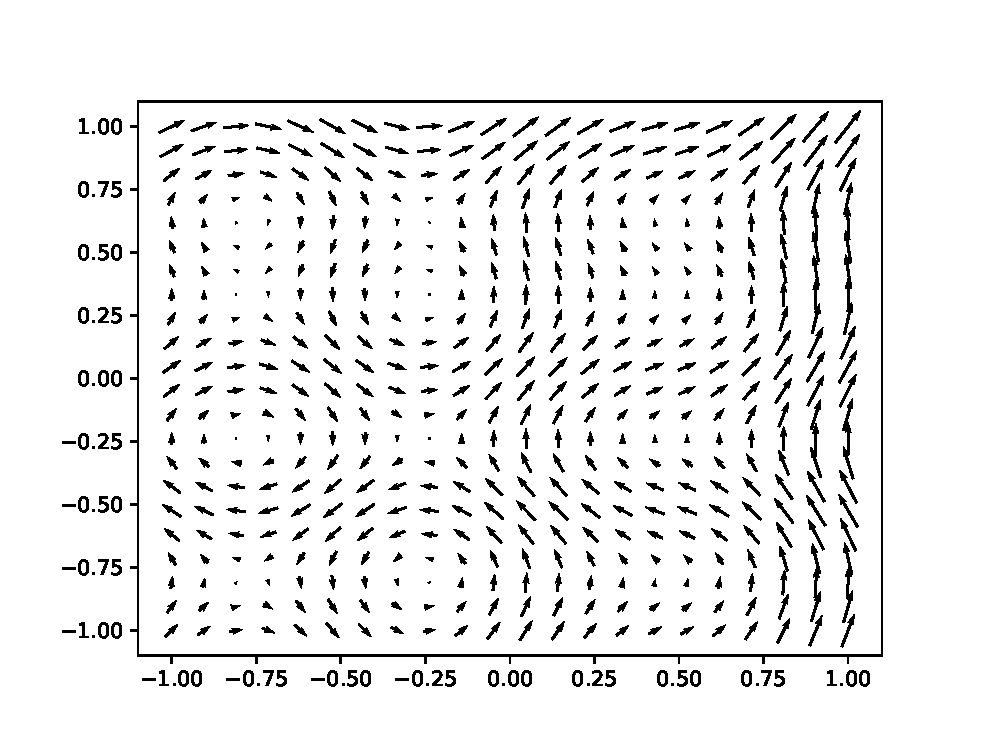
\includegraphics[scale=.40]{first_div_field.eps}&
				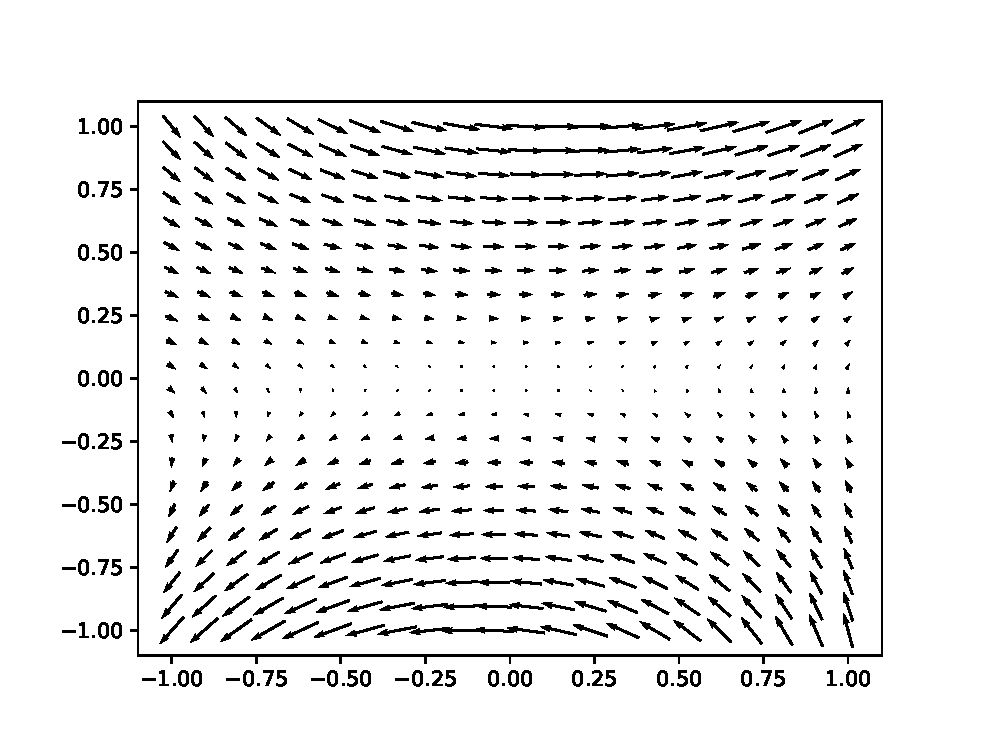
\includegraphics[scale=.40]{second_div_field.eps} \\
				(a) & (b)\\
				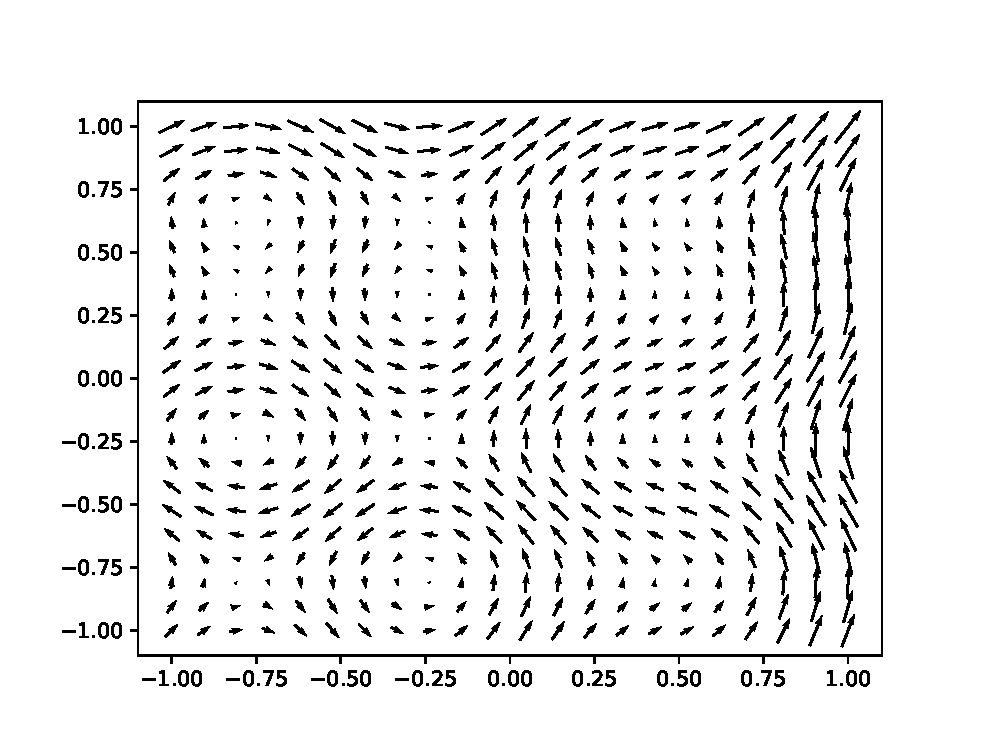
\includegraphics[scale=.40]{first_div_field.eps}&
				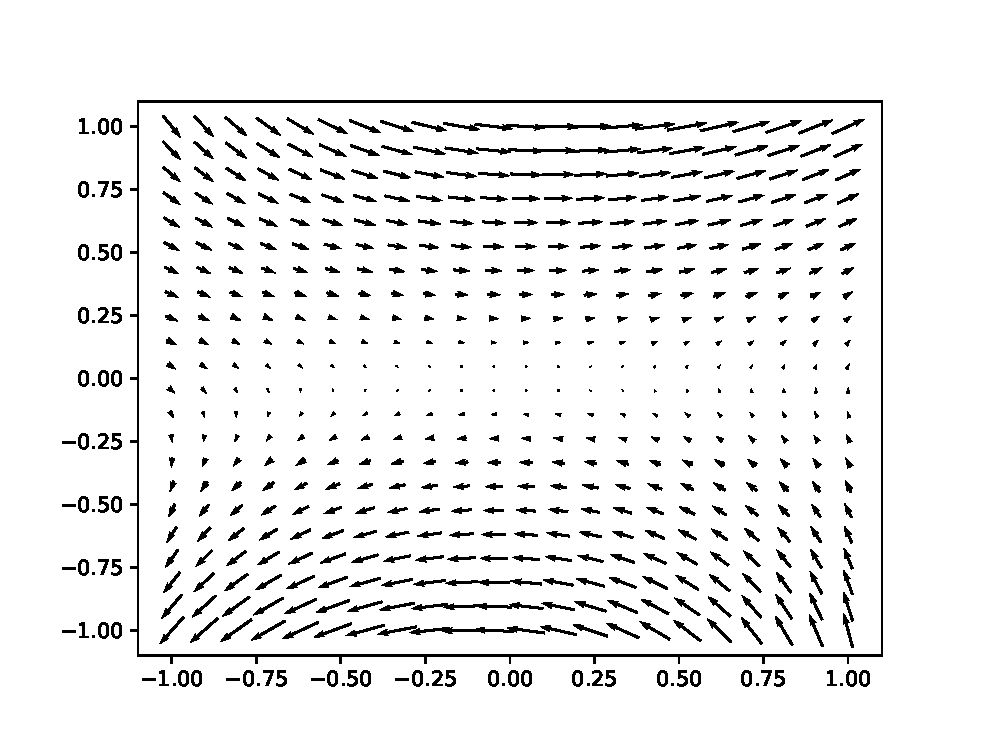
\includegraphics[scale=.40]{second_div_field.eps} \\
				(c) & (d)
			\end{tabular}
		\end{center}
		\caption{Examples of divergence free generated vector fields.
			(a). First class; 
			(b). Second class;
			(c). Third class;
			(d). Fourth class.
			}
		\label{fig:data_ex}
\end{figure}
%%%%%%%%%% end figure %%%%%%%%%%%%%